\section{Evaluation}\label{s:eval}

\FYI{

# EXT4
-
- Score

# F2FS
- Score

# Fragmentation on FDP?
}


\begin{comment}
초반 - 실험 환경 설명
1. free space 측정방법
2. grep test => filesystem aging과 똑같은데.. 괜찮나..? => 그냥 스며들도록?
3. dynamic layout score => 일단은 스며들도록..
4. Git workload
5. RocksDB workload
6. Eval Setup

실험 결과
1. 실제로 노화가 영향을 주나? ext4만 사용하여
			=> latency과 dynamic score를 비교하며, dynamic score과 반비례하여 latency가 증가한다.
			왜 이런 결과가 나오는지? fragmentation 때문인데, 이걸 그림과 대조하며 설명.
			근데 어떤 그림을 사용해야 할지 고민됨.
==> 결론적으로, 아직은 fragmentation문제는 여전하기 때문에, snapshot으로 쉽게 쉽게 하자

2. compare file system => ..? ext4랑 F2FS간 비교를 해야하는데..
=> free space 쪽 그림 바꿔보자

3. dump하는데 필요한 저장공간 => 그래서 update된 storage부분만 snapshot뜨기로 함. => 이건 어느정도?
 	 전체 storage를 dump vs update된 storage만 dump 했을 때의 시간 차이
	 => 큰 차이는 없고 데이터 배치에 따라 결과값이 달라짐.
	 => 굳이 따지면 save는 update된 storage만 dump하는게 조금떠 빠르고 load는 느리게 관측됨
	 => 왜지..?



\end{comment}

% Setup
\subsection{Evaluation Environment}
\begin{comment}
=> NVMEVIRT를 사용한 가상환경에서 실험을 진행함.
=> 컴퓨터의 스펙은 동일하게(mir1의 cpu, mem, storage를 설명), nvmevirt는 conv로, storage의 크기만 다르게 해서 실험을 진행함.
=> nvmevirt가 구현된 커널 스펙
=> Line of code
\end{comment}


We evaluated using two workloads to aging the stroage system.
%  Git workload
The Git aging benchmark\cite{conway:login17,senescence:fast17} can incur aging in a real-world environment that people commonly use.
Git is a distributed version control system that allows synchronization of source code changes.
This benchmark generates workloads by simulating developers working on collaborative projects using Git.
Experiments are conducted using the git pull command, which creates new source files, deletes old files, or modifies files. During this process, Git maintains its internal data structure, leading to filesystem aging.
To measure the extent of aging, multiple git pull commands can be executed, and latency can be measured through reads using grep.

% rocksdb workload


% ext4 file system


% f2fs file system


% Aging affects the performance of storage
\subsection{Aging affects the performance of storage}
\begin{comment}
1. dynamic score를 소개
2. free_block말하면서 free block size가 작아짐을 언급
=> 다른 fragmentation도 소개하고 싶은데..
3. latency를 소개하며, dynamic score와 반비례하게 증가함을 언급
\end{comment}


\begin{figure}[t]
    \centering
	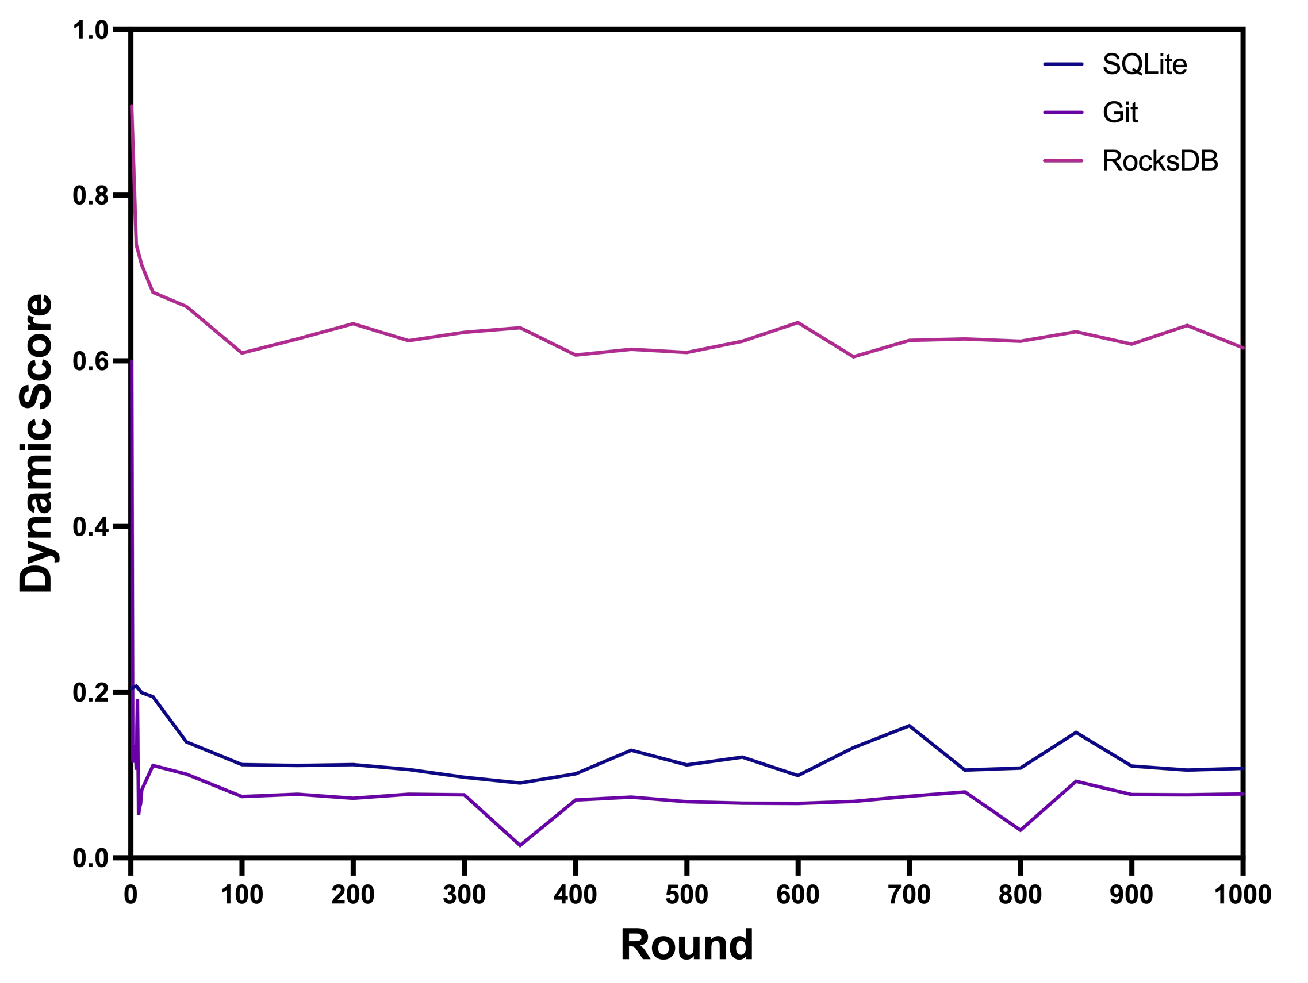
\includegraphics[width=0.95\columnwidth]{graphs/ext4_dynamic}
	\caption{Dynamic Score-EXT4\SK{항목간 누가 누군지 구분이 잘 되지 않아요}}
	\label{f:ext4_dynamic}
\end{figure}

\begin{figure}[t]
    \centering
	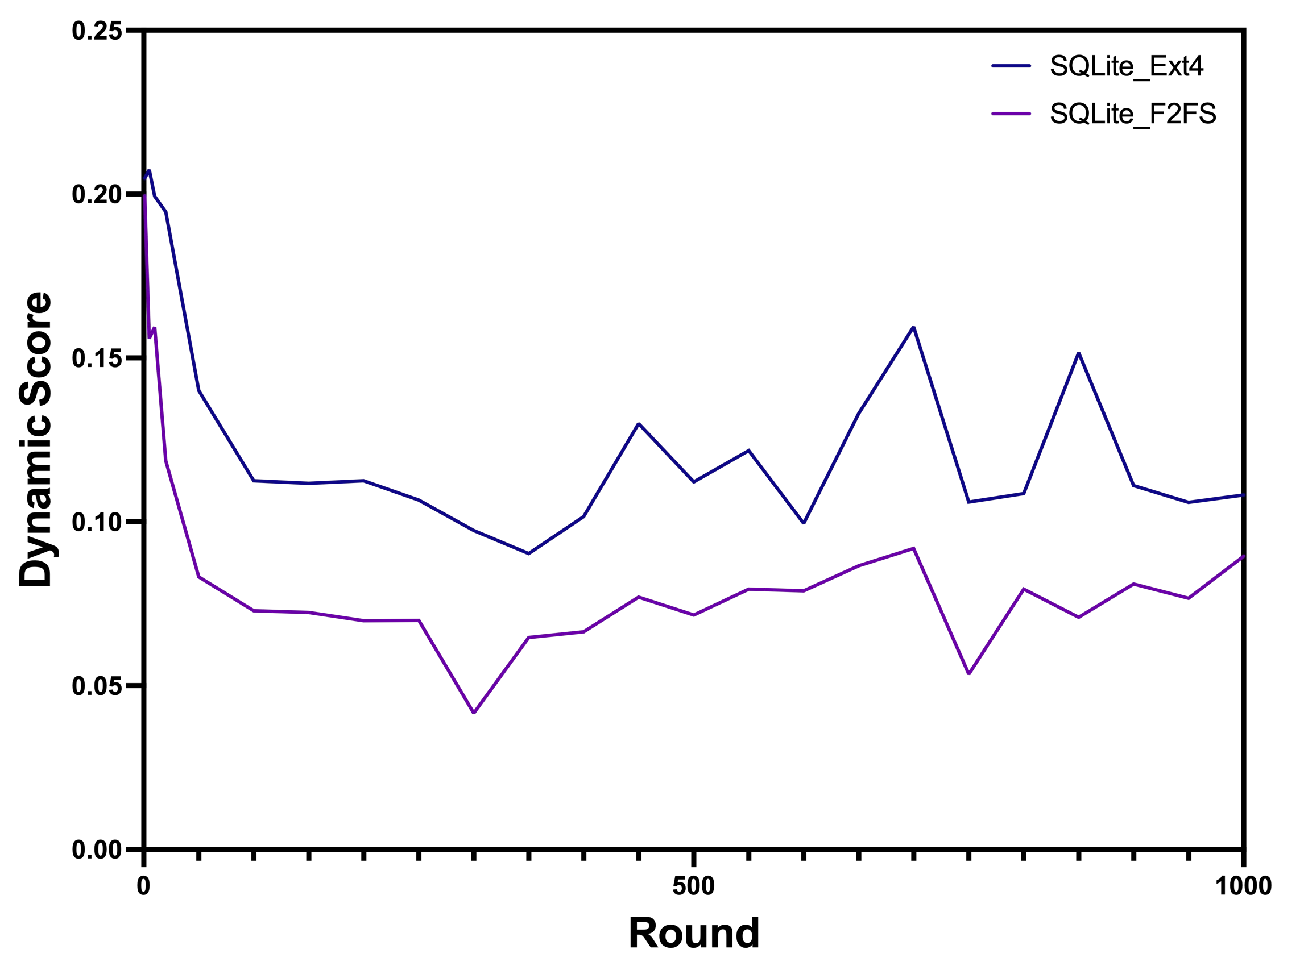
\includegraphics[width=0.95\columnwidth]{graphs/f2fs_vs_ext4_dynamic}
	\caption{Dynamic score of SQLite on F2FS and EXT4}
	\label{f:f2fs_vs_ext4_dynamic}
\end{figure}

% Overall trends
First, we evaluated the fragmentation trends of filesystems using the dynamic layout score as a metric.
The score is computed by analyzing I/O requests captured through \cc{blktrace} and measuring the proportion of contiguous blocks among requested blocks.
A lower dynamic layout score indicates lower contiguity of data and metadata, implying a higher degree of fragmentation within the storage system~\cite{senescence:fast17}.

Figure~\ref{f:ext4_dynamic} shows the change in dynamic layout score over time on the EXT4 filesystem.
As illustrated in the graph, the scores gradually decrease as aging progresses, indicating convergence toward an aged state.
The convergence rates vary depending on the workload, however, in all cases, it takes more than 100 rounds to sufficiently age the filesystem.
This observation highlights the time-consuming nature of traditional aging processes and underscores the utility of our snapshot scheme in rapidly configuring an aged state.

% Aging trends ext4 vs f2fs
The phenomenon of the dynamic layout score decreasing with aging is not unique to EXT4.
Figure~\ref{f:f2fs_vs_ext4_dynamic} compares the behavior of EXT4 and F2FS under the SQLite workload.
F2FS also exhibits a similar trend to EXT4, with the dynamic layout score gradually decreasing over time.


\begin{figure*}[t]
    \centering
	\subfloat[Git]{%
		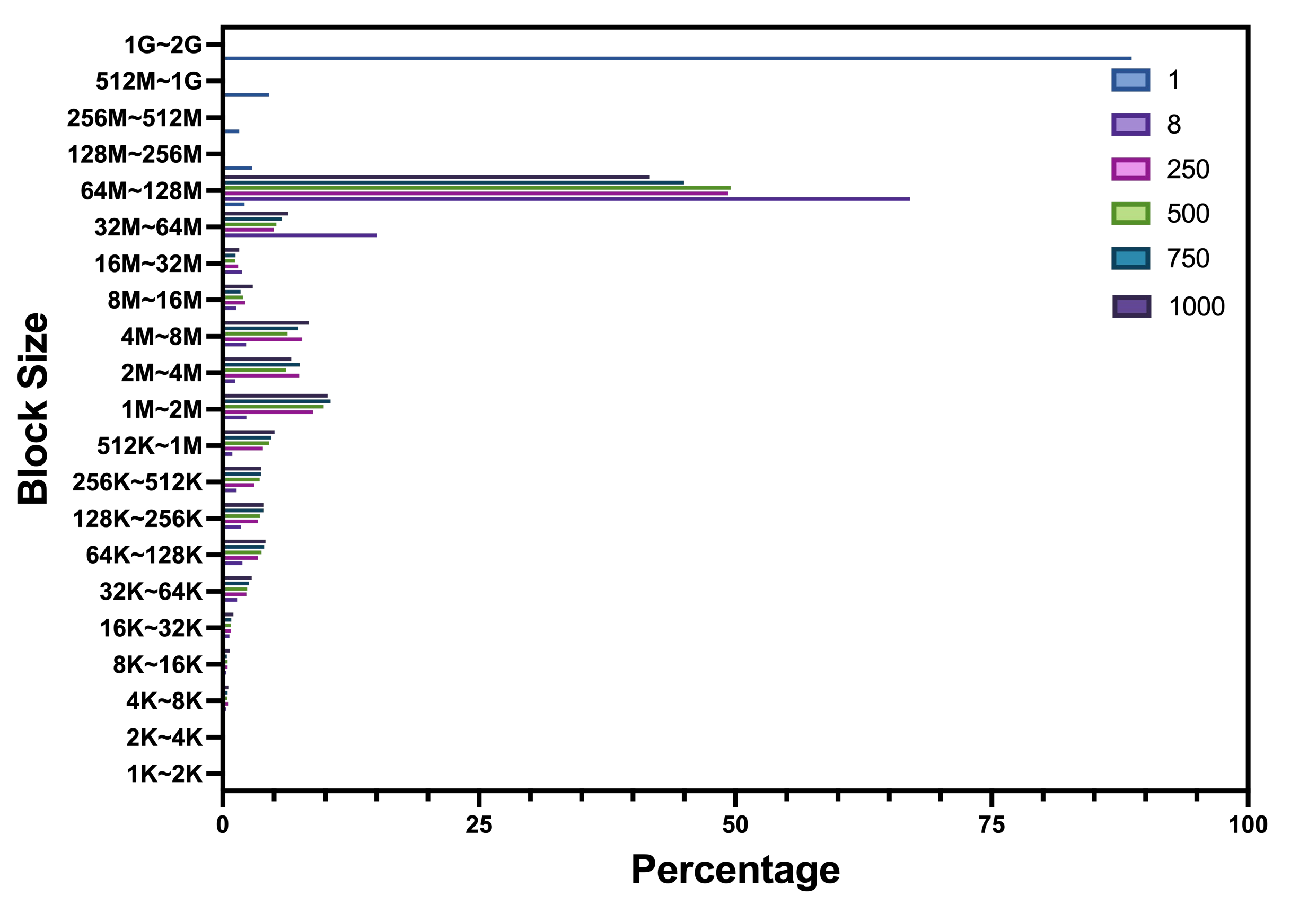
\includegraphics[width=0.95\columnwidth]{graphs/free_block_git}
		\label{f:free_block_git}
	}
	\subfloat[RockDB]{%
		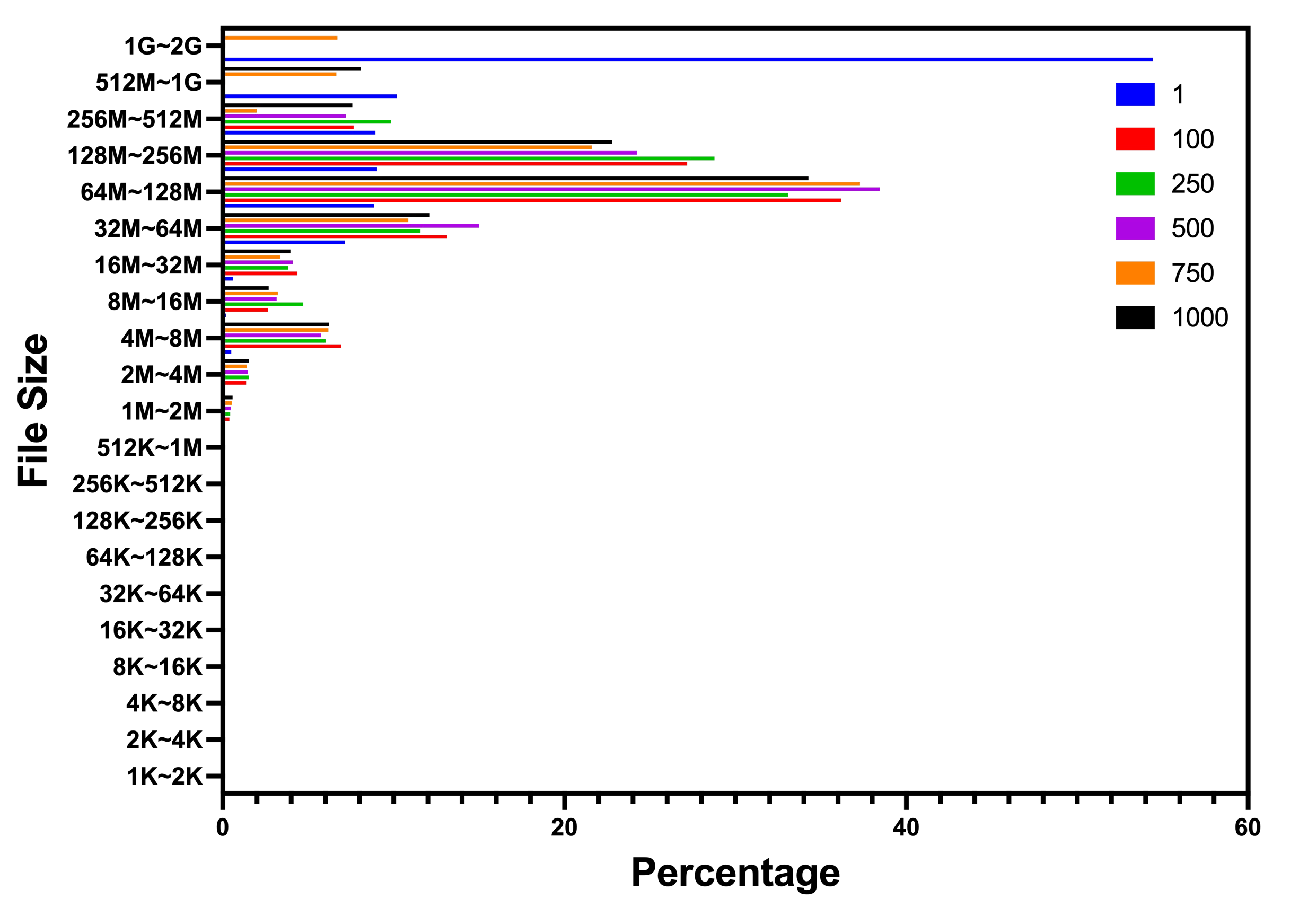
\includegraphics[width=0.95\columnwidth]{graphs/free_block_rocksdb}
		\label{f:free_block_rocksdb}
	}
	\caption{Free block}\label{g:free_block}
\end{figure*}

In our experiment, we also observed fragmentation in the storage.
Figure~\ref{g:free_block} shows the observations \SK{What observation? be specific} for the filesystem when it is EXT4, specifically for the Git and RocksDB workloads.
In both experiments, before aging occurred, the free block sizes were concentrated at 2G and 1G.
However, as aging progressed, the 128M free blocks became the most prevalent, and particularly in the Git workload, free blocks of size 8K were also observed.
This indicates that after aging, the free blocks in the storage became physically dispersed, resulting in the presence of smaller free block sizes compared to before.


\begin{comment}
i want write other fragmentation.
intrfile fragmentation, interfile fragmentation...
\end{comment}


\begin{figure}[t]
    \centering
	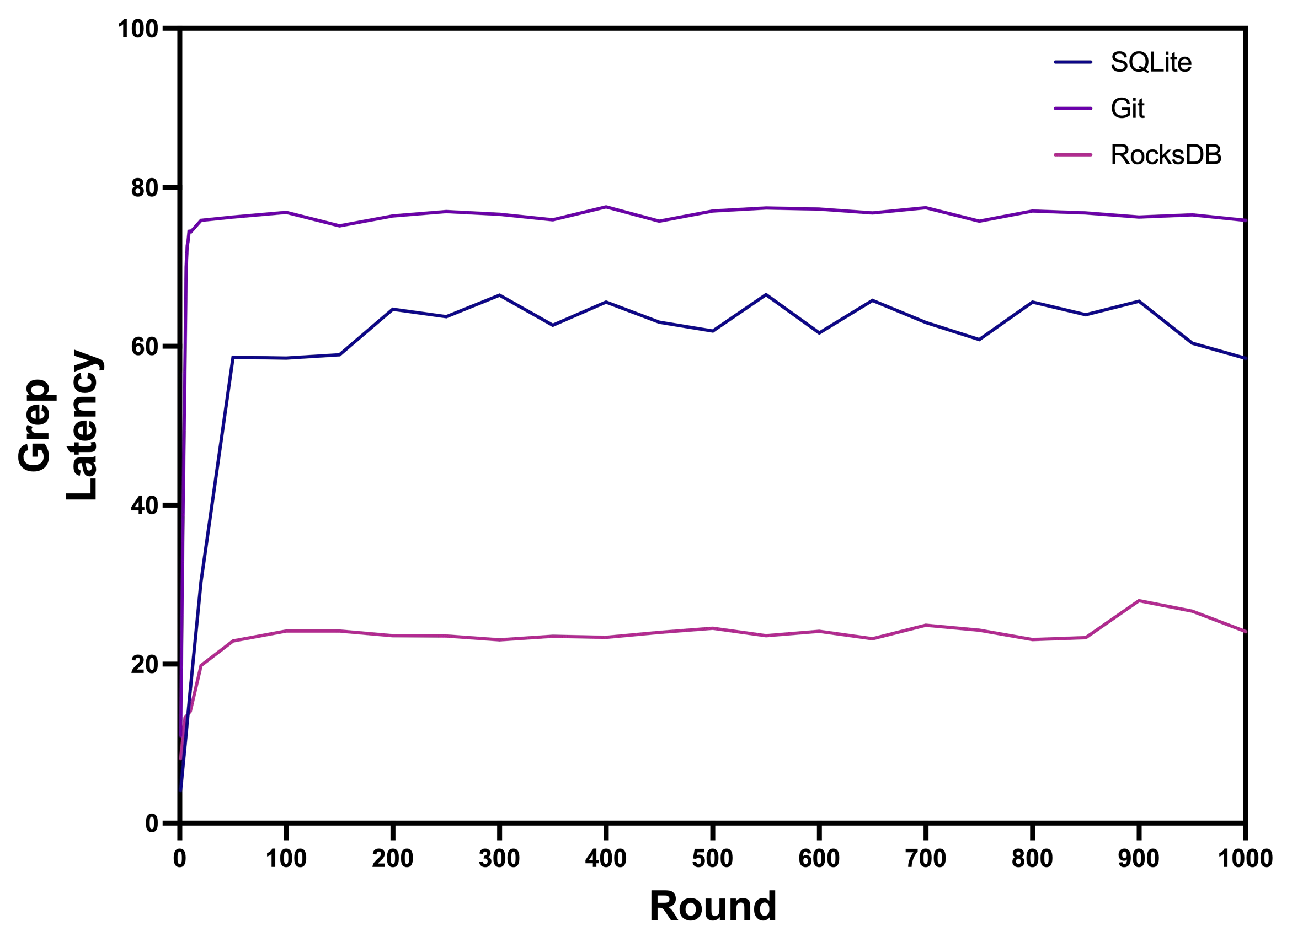
\includegraphics[width=0.95\columnwidth]{graphs/ext_latency}
	\caption{Latency-EXT4}
	\label{f:ext_latency}
\end{figure}

\begin{figure}[t]
    \centering
	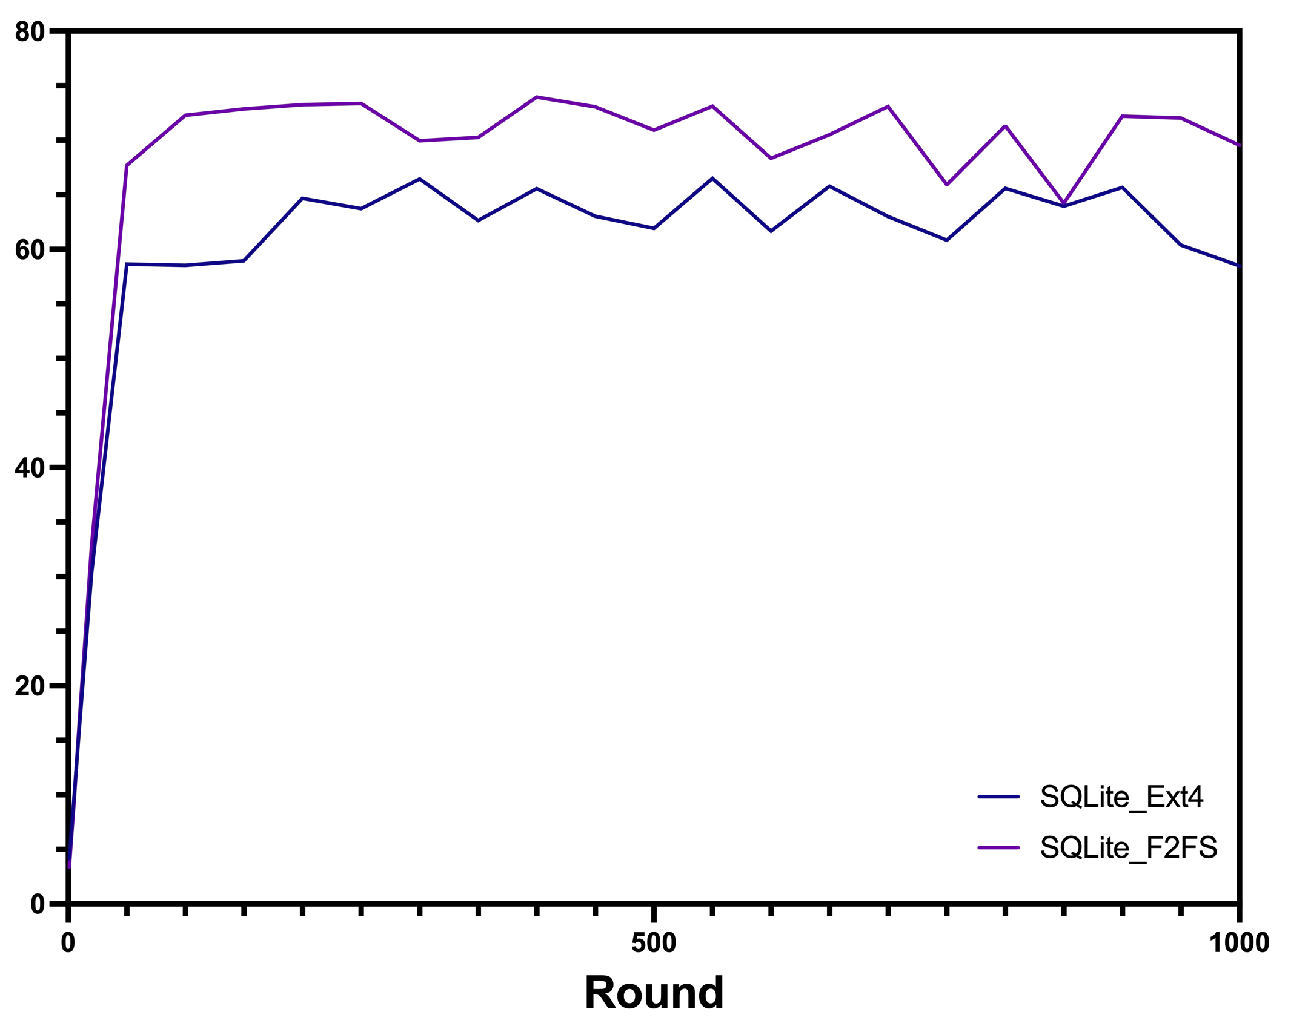
\includegraphics[width=0.95\columnwidth]{graphs/f2fs_vs_ext4_latency}
	\caption{Latency-EXT4 vs F2FS}
	\label{f:f2fs_vs_ext4_latency}
\end{figure}

We have observed that such fragmentation can affect storage performance.
Figure~\ref{f:ext_latency} shows the results of the Grep test conducted in an EXT4 file system environment.
The grep test represents the wall-clock time required to perform a recursive grep in the root directory of the file system.
It demonstrates an increase Grep latency across all workloads.
This is inversely proportional to the results shown by the Dynamic Layout Score.
The Figure~\ref{f:f2fs_vs_ext4_latency} not only in the EXT4 environment but also in the F2FS environment shows the same results.
Still, it indicates that fragmentation in storage has a negative impact on storage performance.

% comparison snapshot latency \subsection{Comparison Snapshot Latency}
[] dumps the storage.
Therefore, if the original contents of a 1TB storage are copied, a 1TB snapshot is created.
However, not all parts of the storage contain data.
[] only dumps the portions of the storage where meaningful data is stored.

\begin{figure}[t]
    \centering
	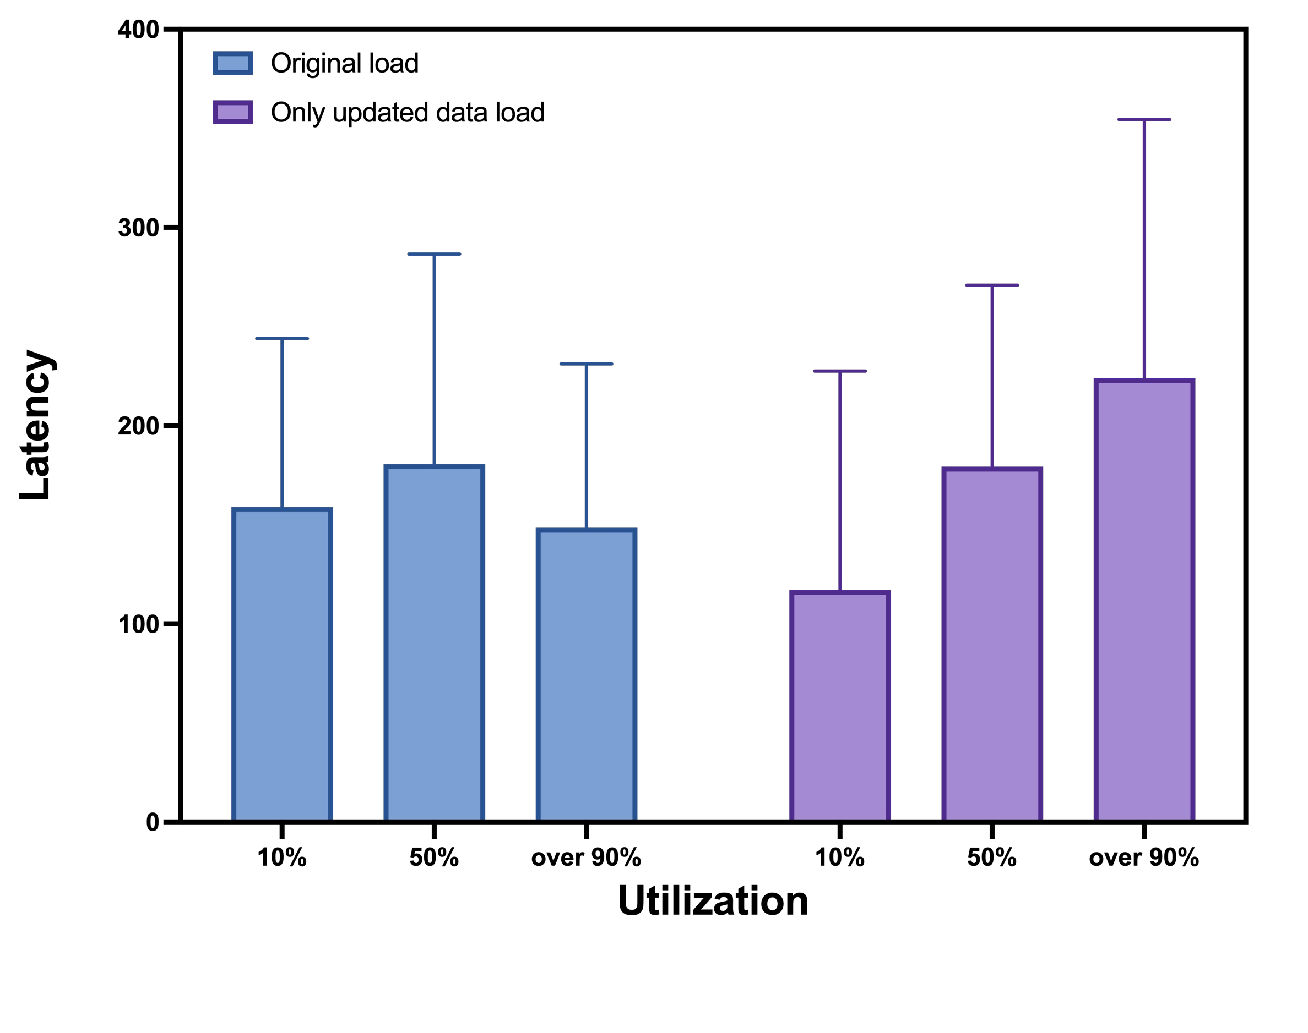
\includegraphics[width=0.95\columnwidth]{graphs/load_latency}
	\caption{Load Latency}
	\label{f:load_latency}
\end{figure}

\begin{figure}[t]
    \centering
	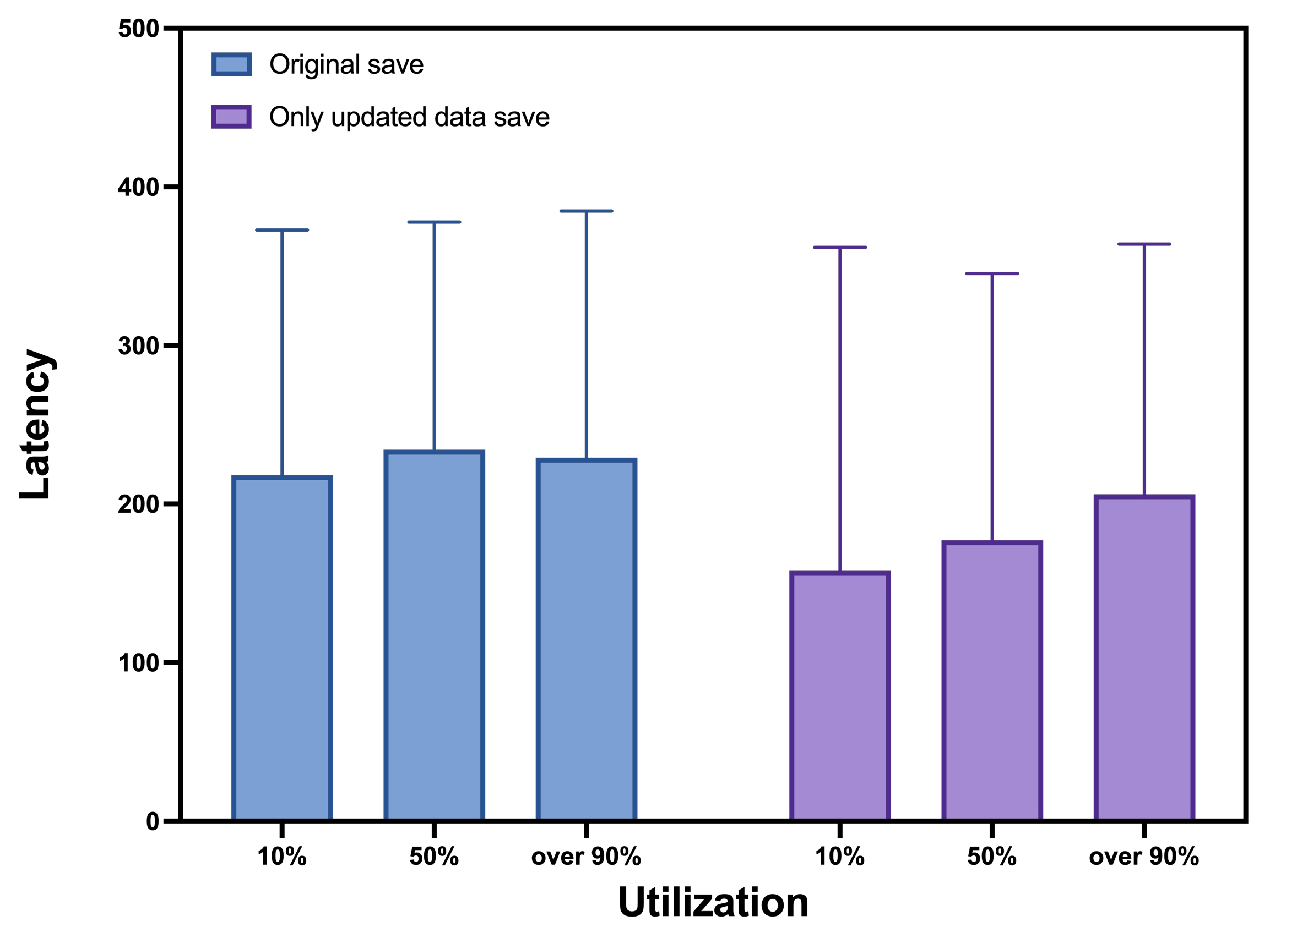
\includegraphics[width=0.95\columnwidth]{graphs/save_latency}
	\caption{Save Latency}
	\label{f:save_latency}
\end{figure}

Figure~\ref{f:save_latency} and \ref{f:load_latency} consider two scenarios: one where the entire storage is dumped and loaded, and another where only the updated data is dumped and loaded.
The results for each scenario, measured at storage utilization levels of 10\%, 50\%, and over 90\%, are presented in bar graphs for storage sizes of 16~GiB, 64~GiB, and 128~GiB.
The thick bars represent the average latency, while the thin lines indicate the maximum values.
A lower position of the lines and bars indicates shorter latency.

When comparing the two scenarios, the case of dumping only the updated data shows slightly lower latency.
However, in the loading scenario, higher latency is observed. This phenomenon arises from the loading method.
To load the updated data, it must be stored at specified addresses in the storage according to the information in the snapshot data.
At this point, the number of load calls can vary depending on the distribution of existing data.
For this reason, there may even be cases where the loading latency is lower.

In the case of saving, similar to loading, the number of save calls varies according to the distribution of stored data.
However, due to caching, the number of save commands reaching the storage device is lower compared to loading.

As shown in the graphs, these differences are not significant.
While dumping the entire storage is more stable in terms of latency, the scenario of dumping only the updated data does not show a large difference in latency.
Rather, the ability to work with a smaller snapshot size presents a greater advantage.


\begin{figure}[t]
    \centering
    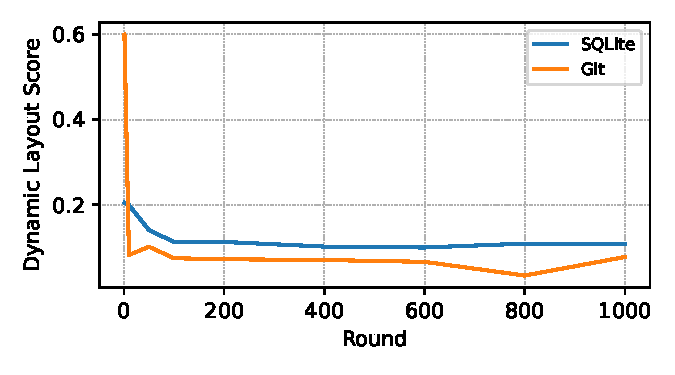
\includegraphics[width=0.95\columnwidth]{graphs/py_graph/dynamic}
    \caption{}
    \label{f:dynamic}
\end{figure}

\begin{figure}[t]
    \centering
    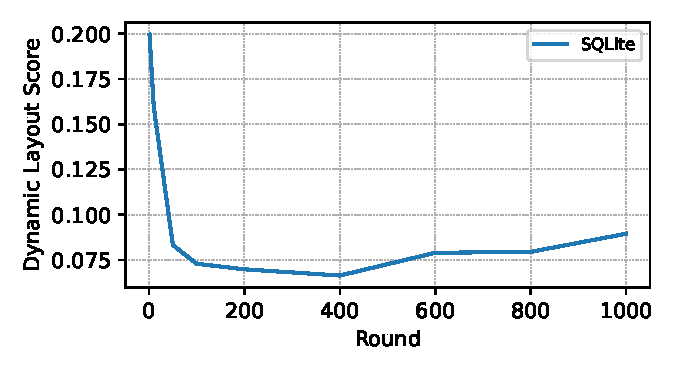
\includegraphics[width=0.95\columnwidth]{graphs/py_graph/dynamic-f2fs}
    \caption{}
    \label{f:f2fs_dynamic_score}
\end{figure}


\begin{figure}[t]
    \centering
    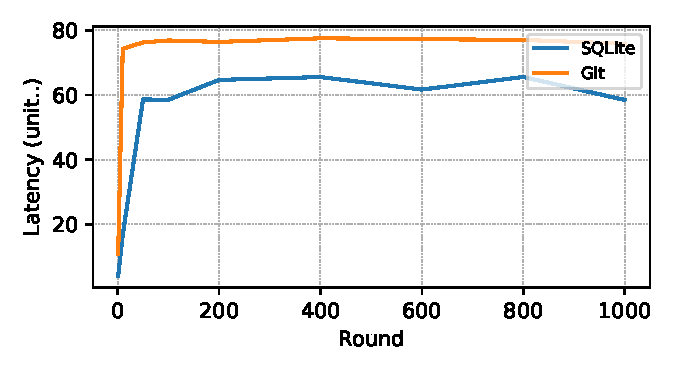
\includegraphics[width=0.95\columnwidth]{graphs/py_graph/latency}
    \caption{}
    \label{f:latency}
\end{figure}

\begin{figure}[t]
    \centering
    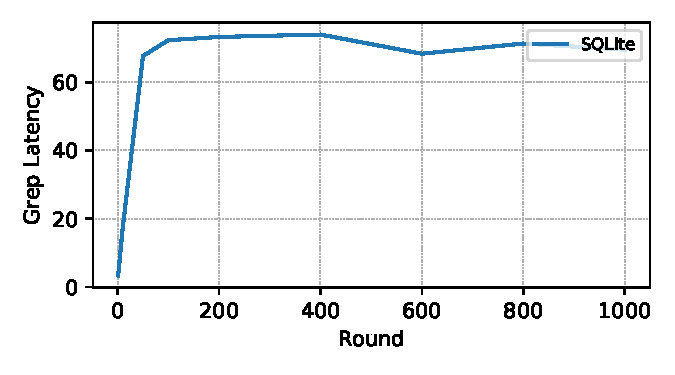
\includegraphics[width=0.95\columnwidth]{graphs/py_graph/latency-f2fs}
    \caption{}
    \label{f:f2fs_latency}
\end{figure}


\begin{figure}[t]
    \centering
	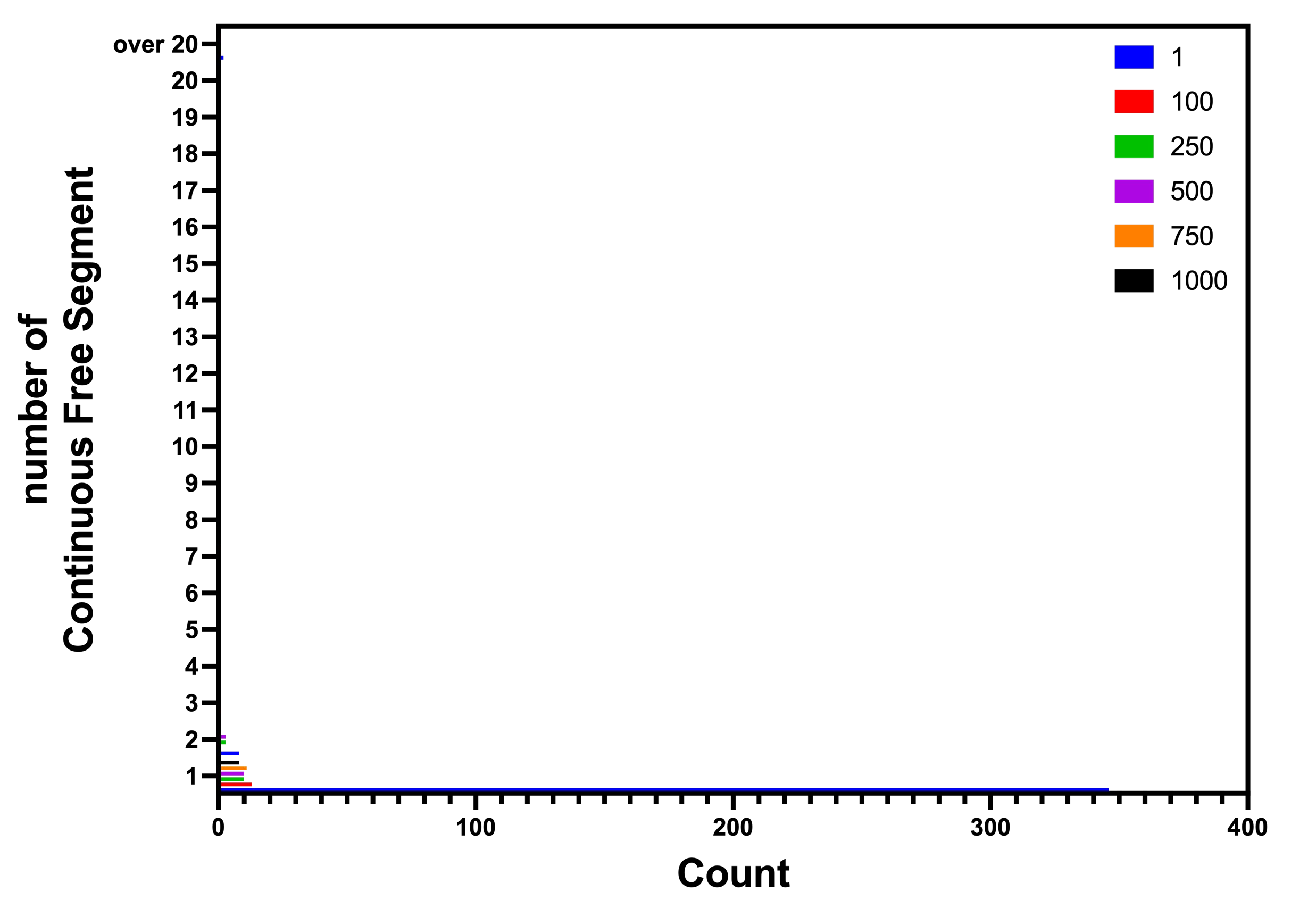
\includegraphics[width=0.95\columnwidth]{graphs/continuous_free_segment_fsfs}
	\caption{Continuous Free Segment-F2FS}
	\label{f:continuous_free_segment_fsfs}
\end{figure}


\begin{figure}[t]
    \centering
	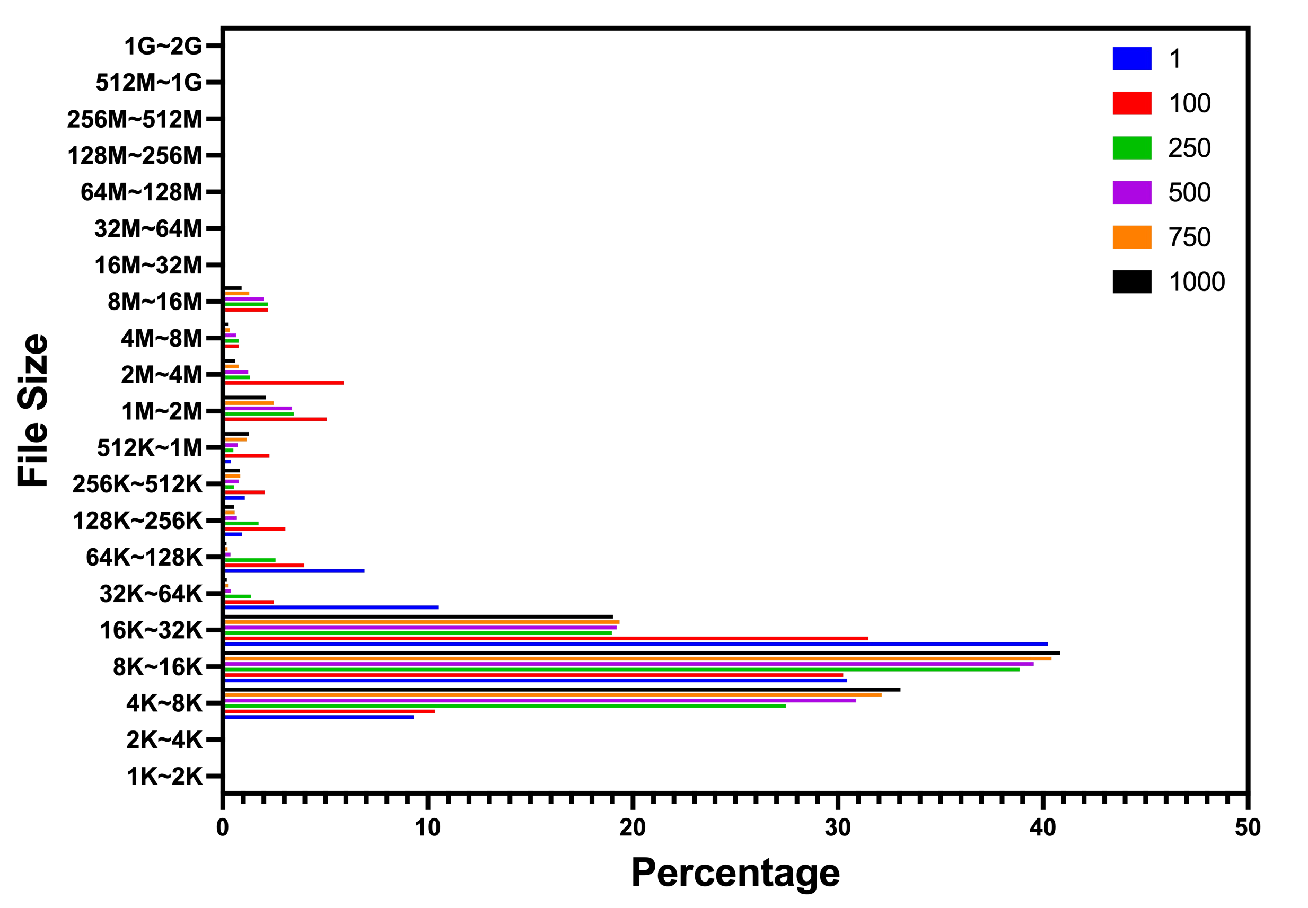
\includegraphics[width=0.95\columnwidth]{graphs/file_block_ext4}
	\caption{File Block-EXT4}
	\label{f:file_block_ext4}
\end{figure}

\begin{figure}[t]
    \centering
	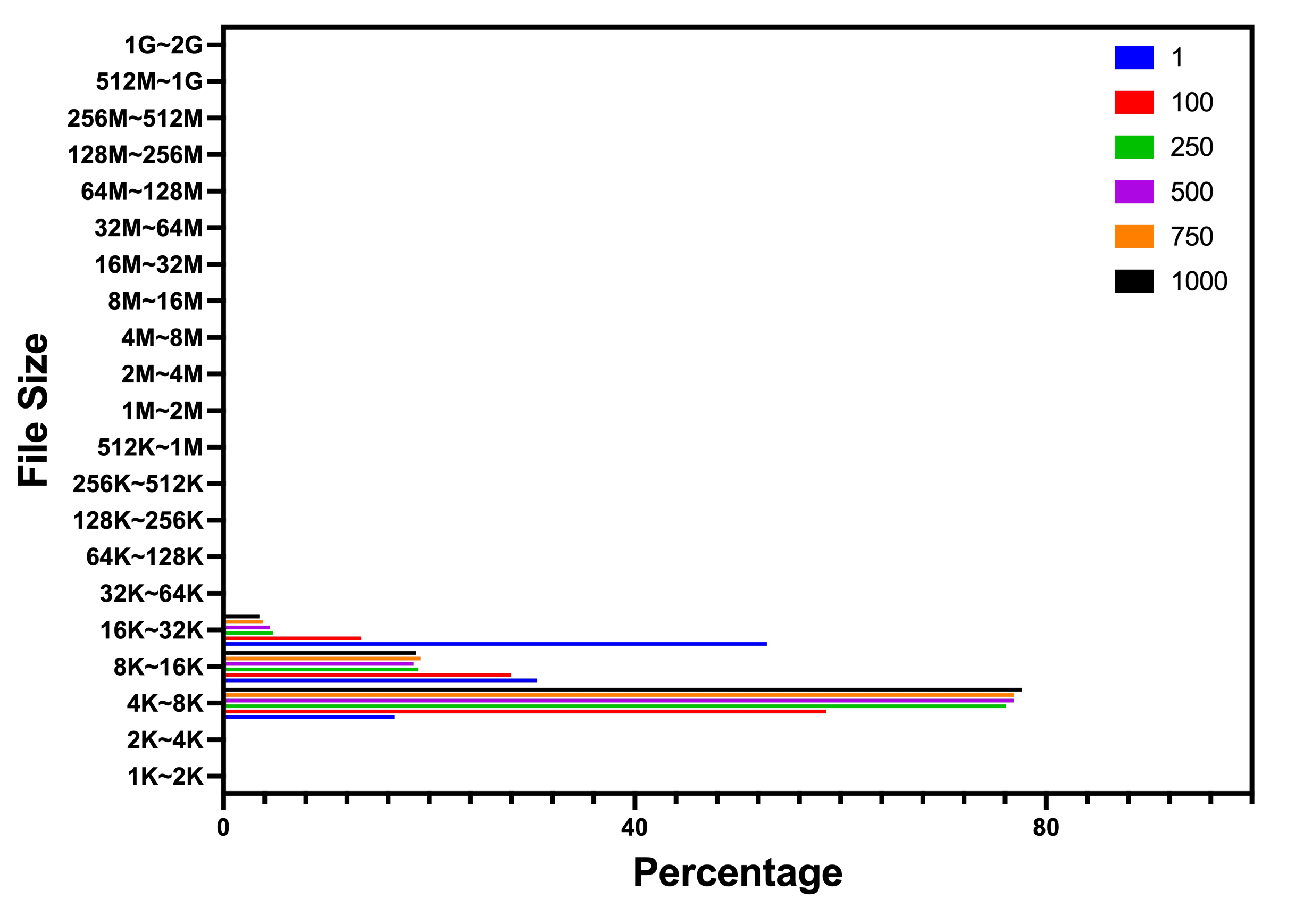
\includegraphics[width=0.95\columnwidth]{graphs/file_block_f2fs}
	\caption{File Block-F2FS}
	\label{f:file_block_f2fs}
\end{figure}

\begin{figure}[t]
    \centering
	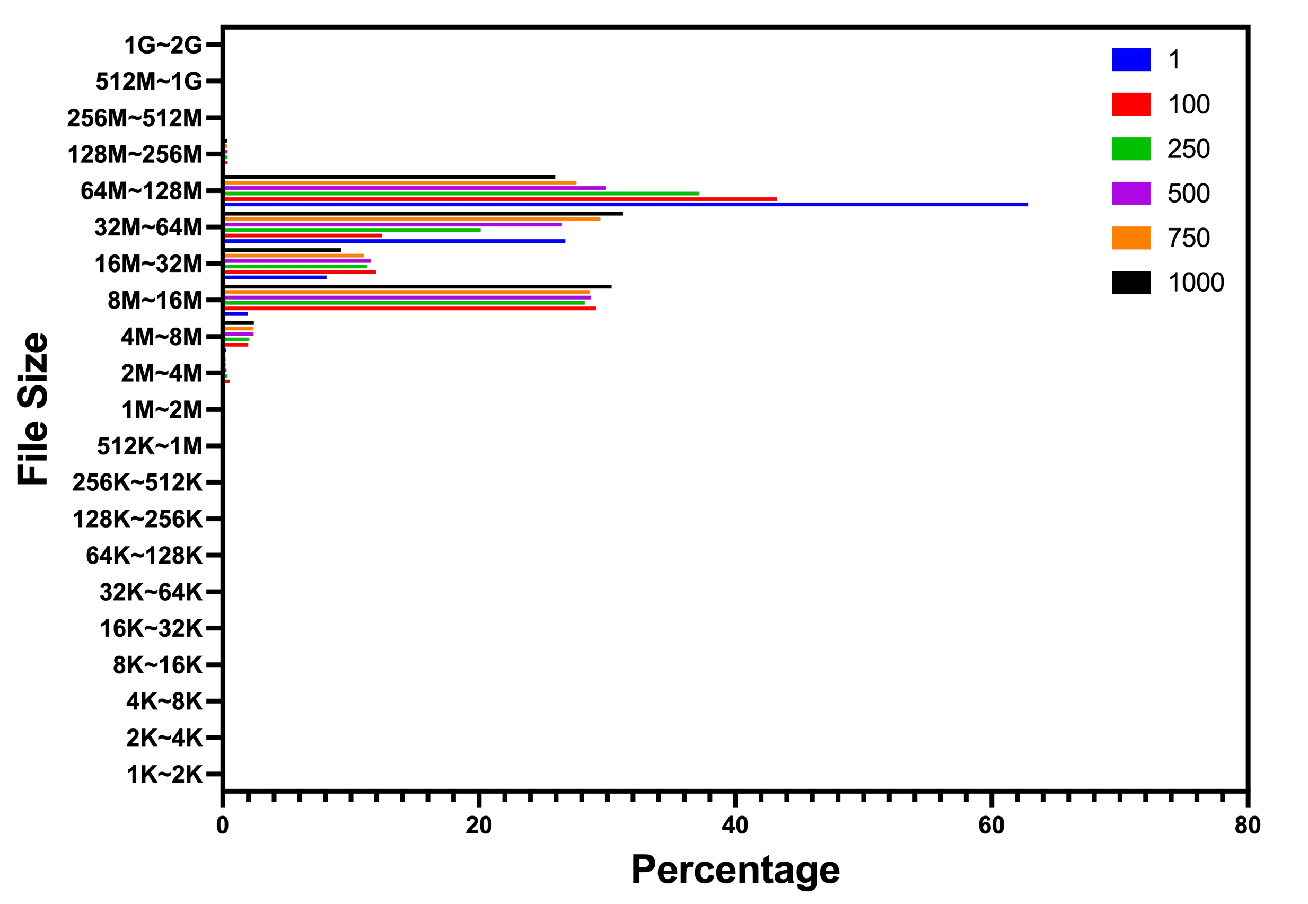
\includegraphics[width=0.95\columnwidth]{graphs/file_block_rocksdb}
	\caption{File Block-RockDB}
	\label{f:file_block_rocksdb}
\end{figure}

\begin{figure}[t]
    \centering
	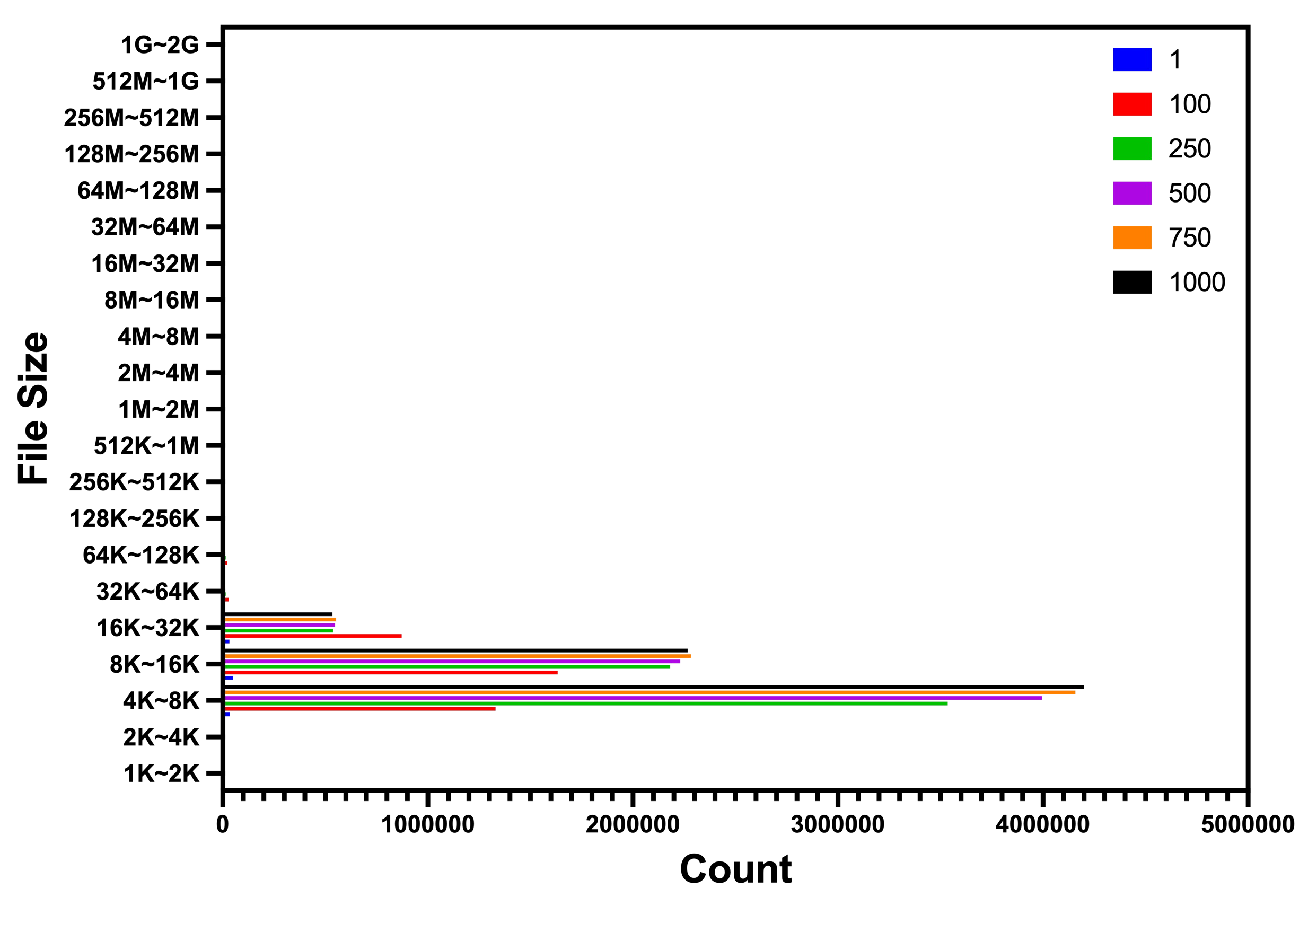
\includegraphics[width=0.95\columnwidth]{graphs/file_extents_ext4}
	\caption{File Extents-EXT4}
	\label{f:file_extents_ext4}
\end{figure}

\begin{figure}[t]
    \centering
	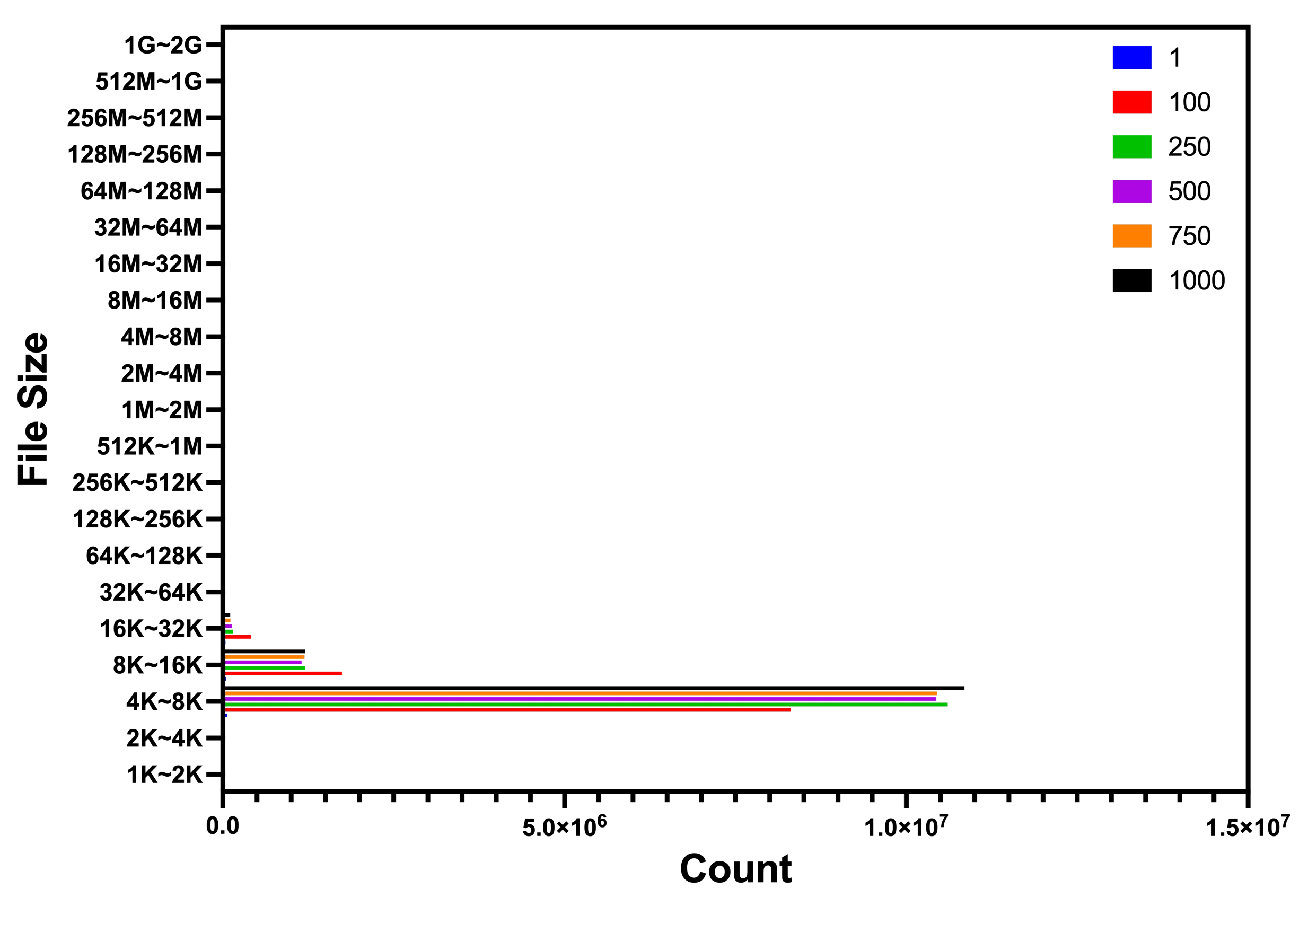
\includegraphics[width=0.95\columnwidth]{graphs/file_extents_f2fs}
	\caption{File Extents-F2FS}
	\label{f:file_extents_f2fs}
\end{figure}

\begin{figure}[t]
    \centering
	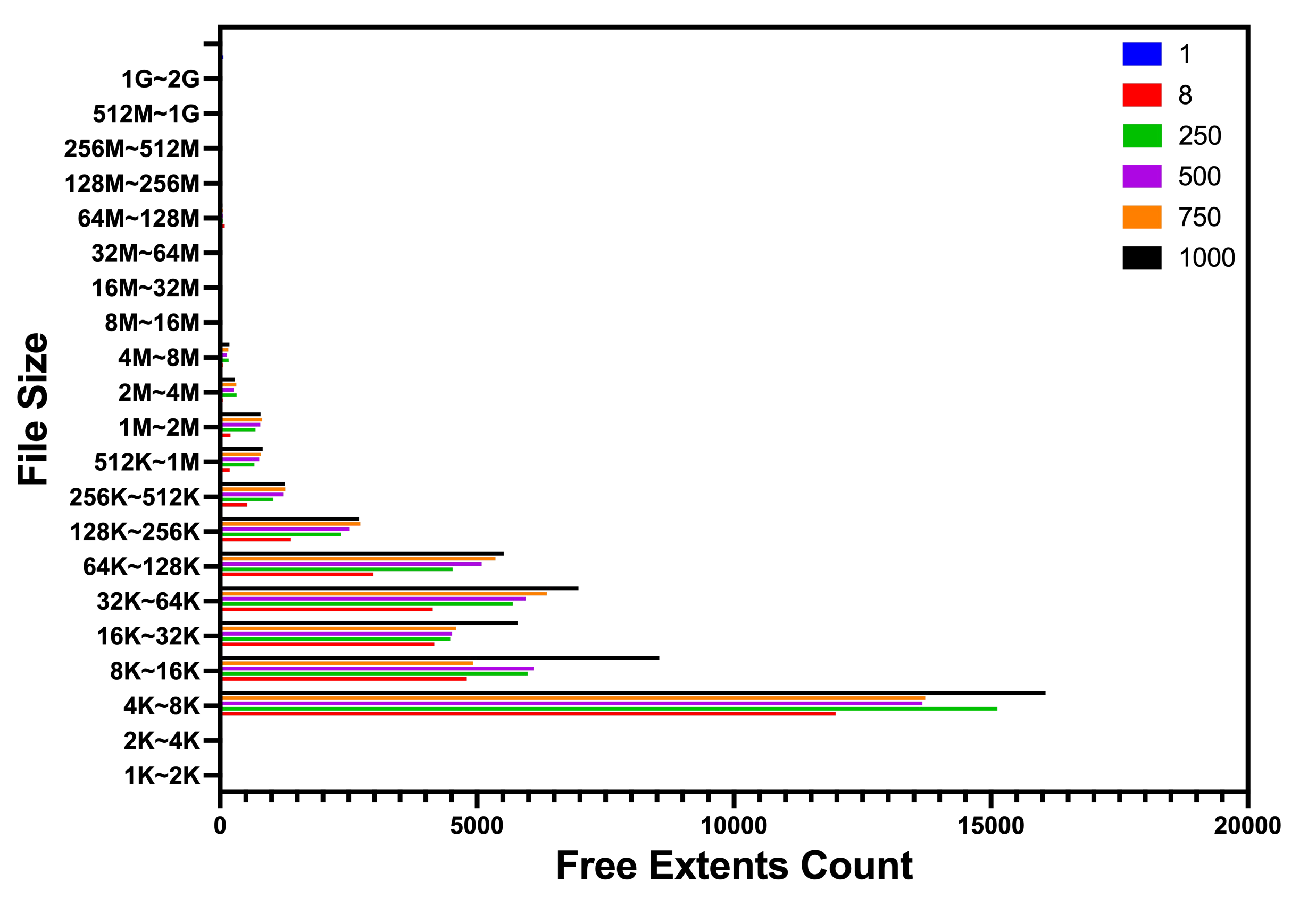
\includegraphics[width=0.95\columnwidth]{graphs/file_extents_git}
	\caption{File Extents-GIT}
	\label{f:file_extents_git}
\end{figure}

\begin{figure}[t]
    \centering
	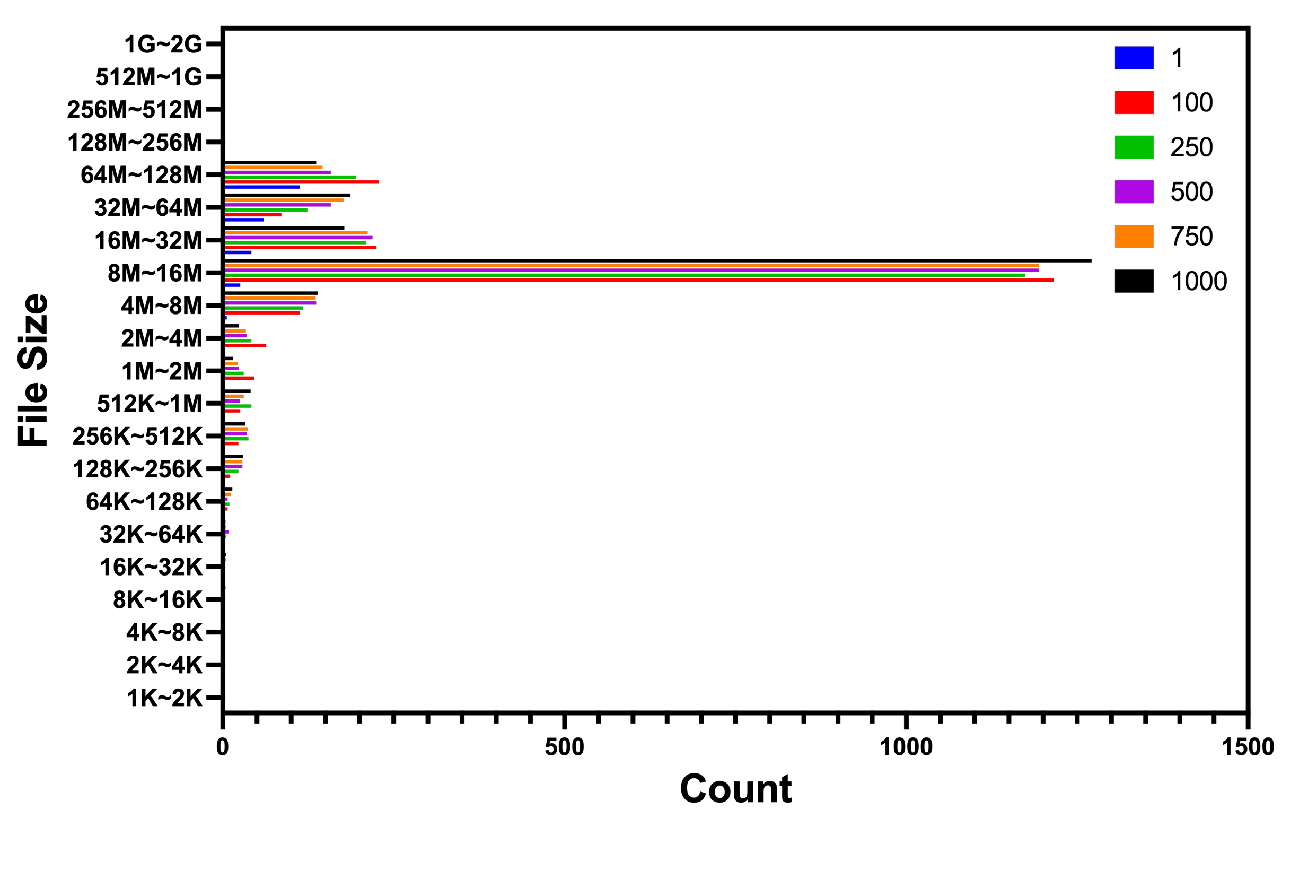
\includegraphics[width=0.95\columnwidth]{graphs/file_extents_rocksdb}
	\caption{File Extents-RocksDB}
	\label{f:file_extents_rocksdb}
\end{figure}

\begin{figure}[t]
    \centering
	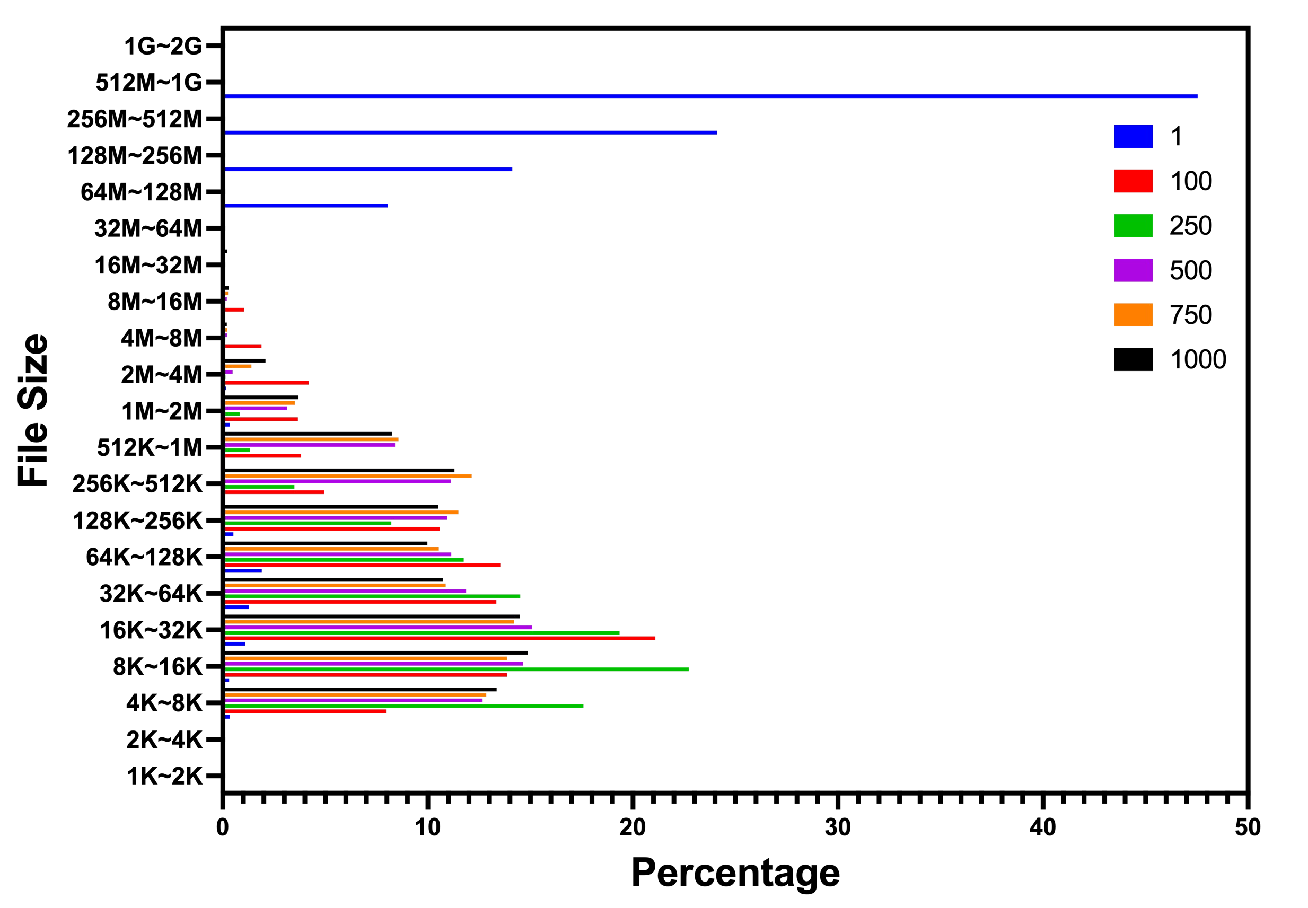
\includegraphics[width=0.95\columnwidth]{graphs/free_block_ext4}
	\caption{Free Block-EXT4}
	\label{f:free_block_ext4}
\end{figure}


\begin{figure}[t]
    \centering
	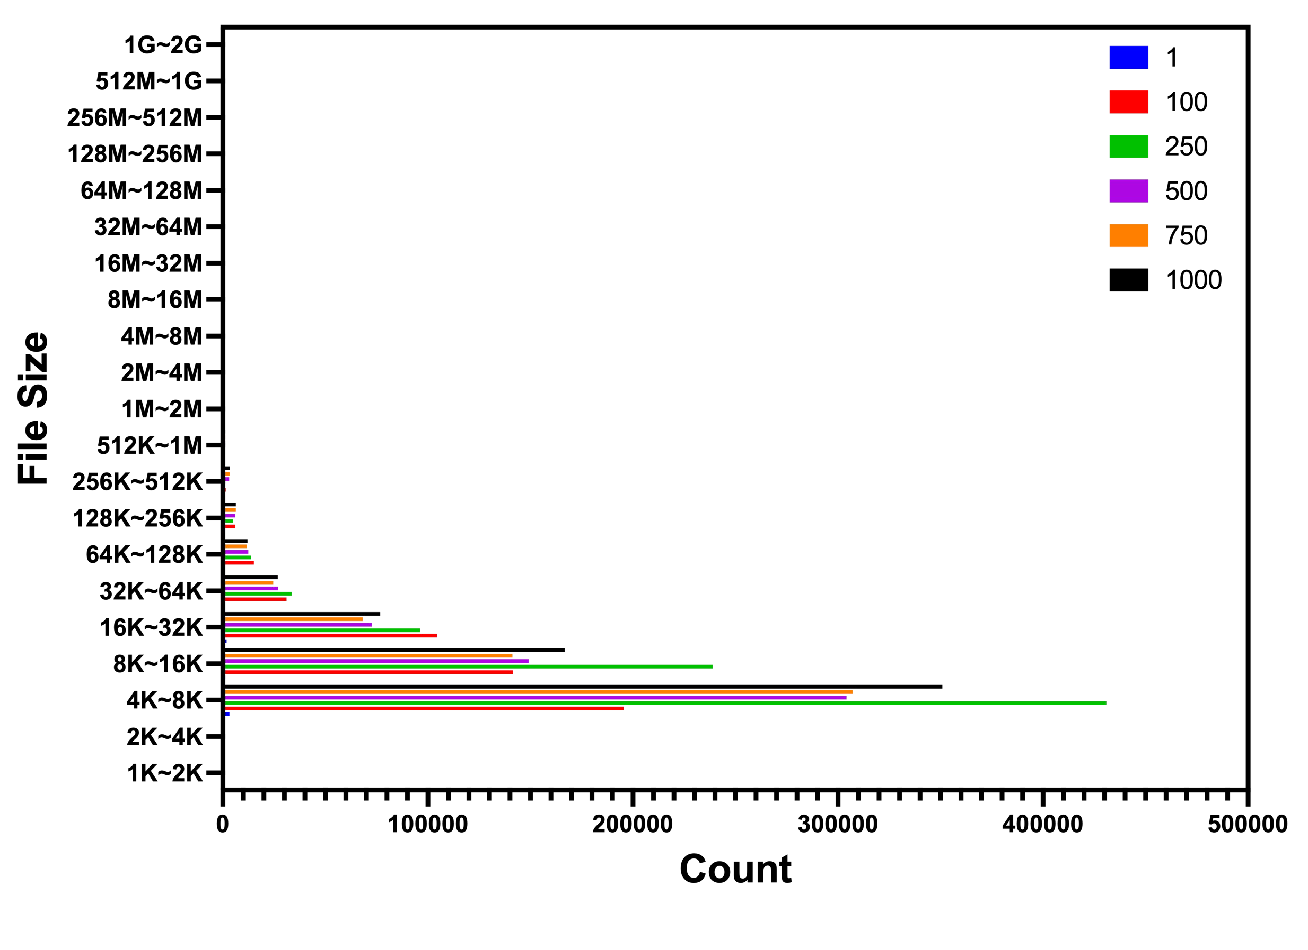
\includegraphics[width=0.95\columnwidth]{graphs/free_extents_ext4}
	\caption{Free Extents-EXT4}
	\label{f:free_extents_ext4}
\end{figure}

\begin{figure}[t]
    \centering
	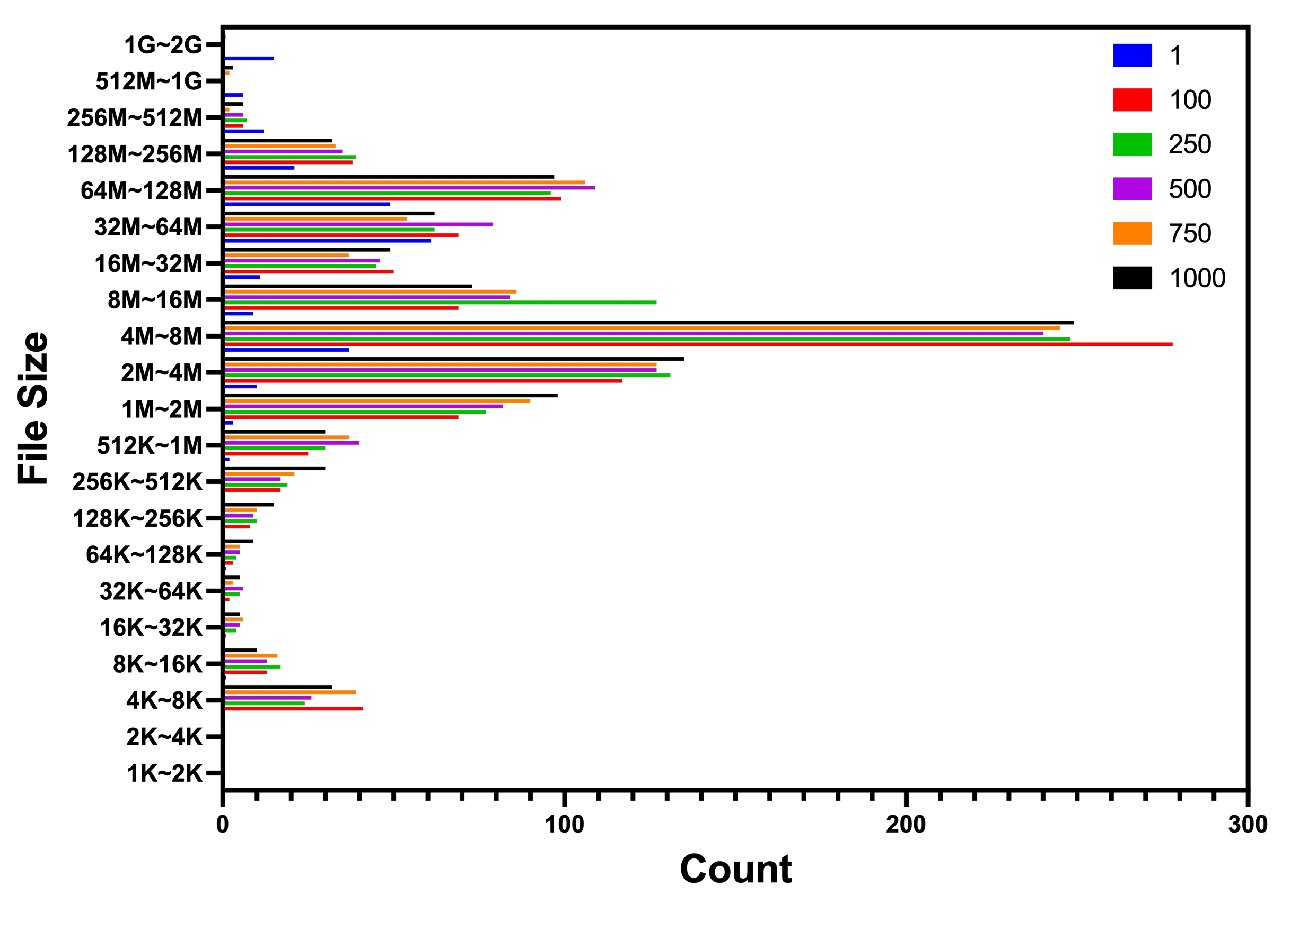
\includegraphics[width=0.95\columnwidth]{graphs/free_extents_rocksdb}
	\caption{Free Extents-RockDB}
	\label{f:free_extents_rocksdb}
\end{figure}

\begin{figure}[t]
    \centering
	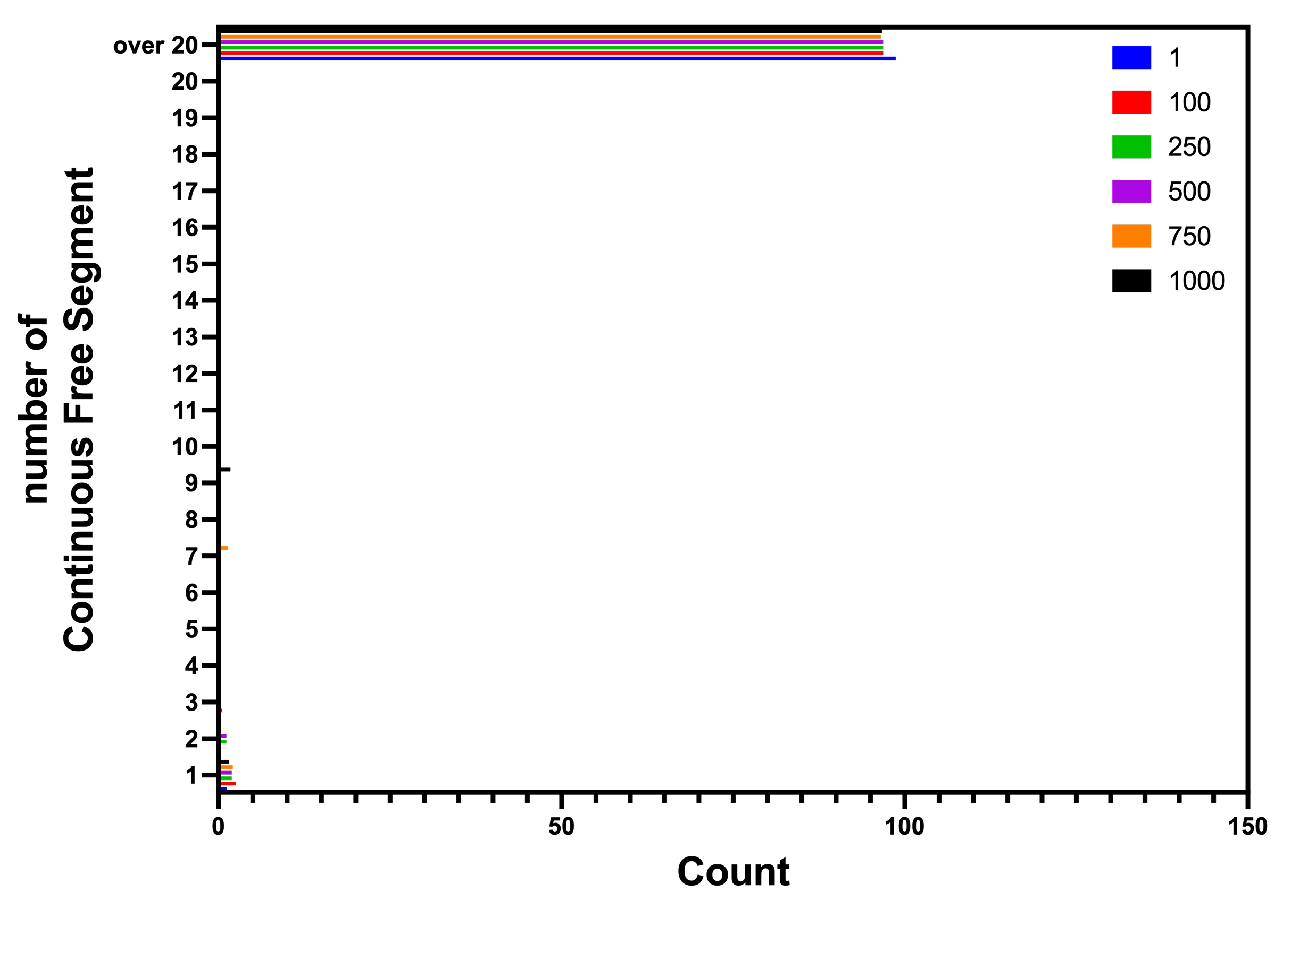
\includegraphics[width=0.95\columnwidth]{graphs/free_segment_f2fs}
	\caption{Free Segment-F2FS}
	\label{f:free_segment_f2fs}
\end{figure}

